\documentclass[10pt,a4paper]{report}

\usepackage[utf8]{inputenc}
\usepackage{amsmath}
\usepackage{amsfonts}
\usepackage{amssymb}
\usepackage{graphicx}
\usepackage{color}
\usepackage{enumitem}
\usepackage[top=1cm, bottom=2cm, left=2cm, right=2cm]{geometry}

\usepackage{fancyhdr}
\pagestyle{fancy}

\fancyhead{}
\fancyfoot{} 
\lhead{ \hspace{0.1cm} M1 WI 2014-2015  \hspace{0.4cm} \vline}
\chead{METEOR}
\rhead{K.B - K.L - N.R}
\rfoot{\thepage}

\author{Kevin BASCOL, Kevin LAOUSSING, Nicolas REYNAUD}
\title{METEOR : \\ \vspace*{0.5cm} Le jeu de Dames}

\makeatletter
\renewcommand{\thesection}{\@arabic\c@section}
\makeatother

\begin{document}

\makeatletter
	\begin{titlepage}
	
	\centering
		{
		\vspace*{5cm}
		\hrule height 2pt
		\vspace{0.7cm}
		\Huge \textbf{\@title}}\\
		\vspace{0.7cm}
		\hrule height 2pt
		
		\vfill
		\vspace{1cm}
		\@author\\
		\end{titlepage}
\makeatother
\setcounter{secnumdepth}{4}
\setcounter{tocdepth}{3}
\renewcommand{\contentsname}{Sommaire}
\begingroup\makeatletter
\def\@makeschapterhead#1{%
  {\parindent \z@ \raggedright
    \normalfont
    \interlinepenalty\@M
    \Huge \bfseries  #1\par\nobreak
    \vskip 20pt% <---- à réduire pour avoir plus de place
  }}\makeatother
\tableofcontents
\endgroup
\thispagestyle{empty}
\setcounter{page}{0}
\newpage

\newgeometry{top=2cm, bottom=2cm, left=2cm, right=2cm}

\section{Introduction}
	Notre projet de METEOR consister à implémenter un jeu à 2 joueurs. Nous avons choisi d'implémenter le jeu de Dames, un jeu suffisamment complexe et qui nous laisse apprécier l'efficacité de nos algorithmes.
Nous avons implémenter dans un premier temps l'affichage, les mouvements et les actions du jeu. Puis dans un second temps les règles et spécificité du jeu. Enfin une intelligence artificielle qui se base sur l'algorithme du MinMax, et de 3 fonctions heuristiques.
\section{Le jeu de Dame}
	\subsection{Description}
	Les dames ou jeu de dames est un jeu de société combinatoire abstrait pour deux joueurs où le but est de capturer ou d'immobiliser les pions de l'adversaire.
	\subsection{Configuration du jeu}
	Il existe plusieurs configuration du jeu de dames, pour notre projet nous avons choisi celle-ci :
	\begin{itemize}[label = $\blacktriangleright$]
		\item Damier :  10 x 10.
		\item Nombre de pions par camps : 20.
	\end{itemize}
	
	\subsection{Spécificités et règles de jeu implémentées}
		\subsubsection{Spécificités}
		
		\begin{itemize}[label = $\blacktriangleright$]
		\item Déplacement de pions.
		\item Déplacement de reines.
		\item Transformation de pions en reines.
		\end{itemize}
		
		\subsubsection{Règles de jeu implémentées}
		
		\begin{itemize}[label = $\blacktriangleright$]
		\item Les prises se font à l'avant et à l'arrière.
		\item La dame prend à quelque distance que ce soit, toute pièce suivie d'une ou plusieurs cases vides.
		\item Le deplacement des pions et reines ne sont autorisé que sur des cases colorées.
		\end{itemize}
\section{Algorithme du MinMax}

\section{Heuristiques}

	\subsection{Avantage du nombre de pions}
	 C'est pas ma guerre !

	\subsection{Avantage des positions stratégiques}
		Dans cette heuristique nous avons choisi de donner des valeurs aux cases en fonction de leurs emplacement sur le damier. Les valeurs sont distribuées de la façon suivante:
		\begin{center}
			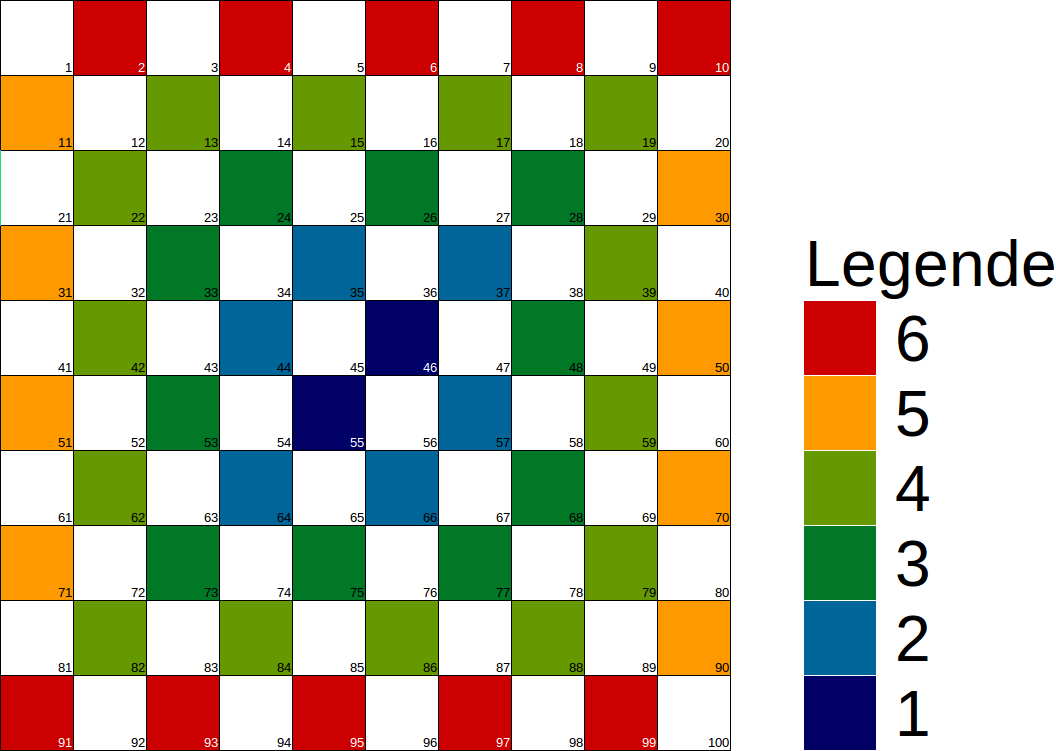
\includegraphics[scale=0.2]{valeursDamier.png}
		\end{center}
		Les cases les plus intéressantes sont celles du haut, pour créer des dames, et celles du bas, pour empêcher l'adversaire de le faire. Ensuite viennent les bordures permettant aux pions d'être hors d'atteinte de l'adversaire. Après on décrémente en se rapprochant du centre du plateau où il est plus facile de se faire prendre un pion.
		L'évaluation d'un instant du jeu se fait alors en ajoutant les valeurs des cases des pions de l'ordinateur, auxquelles on soustrait 10 pour chaque pion adverse pour respecter la règle de la prise obligatoire.
	\subsection{Avantage sur la fragilité défensive adverse }
	Celle là malheureuse si !
\section{Remarques et difficulté}

\section{Conclusion}



\end{document}
